\documentclass[a4j,twocolumn,10pt]{jarticle}
\usepackage[dvipdfmx]{graphicx}
\usepackage{url}
\usepackage{color}
\usepackage[dvipdfmx]{hyperref}

\title{ミーティング資料}
\author{藤井敦寛}
\date{\today}


\begin{document}
\maketitle

\section{進捗状況}
LCDに文字表示完了,一応ヘルメットとの同期もできそう,試行錯誤中.論文の方向を相談したいです.\\
あとは行動認識してました.



\section{今週のアイデア}
\begin{itemize}
  \item なし
\end{itemize}

\section{先週までのキープ案}
\begin{itemize}
  \item 歯の裏トラックパッド
\end{itemize}


\section{ボツ案}
\begin{itemize}
  \item 物理フリックキーボード
  \item プロジェクターのスクリーンをタッチパネル化
  \item 警報音の目的判別
  \item あおり運転に繋がるドライバーの行動変化
  \item ドライバーの疲労度(腕の下がり)
  \item ライダーの疲労度変化(風圧,気温)
  \item グリップ内蔵型スイッチボックス
  \item 次世代型エンジンスタートシステム(ハンドル圧での認証,ドアノブ圧認証)
  \item 次世代型給油停止システム(センサ型)
  \item 人の歩幅を使った何か…疲労度とか?
  \item センサーで眼を観察して動きなどから視力低下限界警告
  \item 1km以上追越車線を走行した場合のアラートと,車線変更可能位置の誘導などの運転支援
  \item 硬筆文字のデジタル化
\end{itemize}

\begin{figure*}[t]
  \begin{center}
    \includegraphics[width=1\textwidth]{Figure_1.eps}
    \caption{}
    \label{fig}
  \end{center}
\end{figure*}

\end{document}
